% ===============================================================
%  جلسه پنجم
% ===============================================================
\chapter{مثالی از استقلال شرطی و گراف‌های تصادفی}

\section{مثال از استقلال شرطی (حل مسئله دو سکه)}

صورت مسئله را در جلسه قبل (مثال \ref{ex:twocoins}) دیدیم: دو سکه با احتمال شیر ۰٫۲۵ و ۰٫۸، یکی به تصادف انتخاب می‌شود، ۵ پرتاب در گزارش $A$ و ۵ پرتاب بعدی در گزارش $B$ ثبت می‌شود. اگر $A=HHTHT$ باشد، احتمال $B=TTHTT$ چقدر است؟

\subsection*{نمادگذاری \lr{(notation)}}
به رشته ۵تایی نخست $S_1$ و به رشته دوم $S_2$ می‌گوییم. سکه نخست را با $C_1$ (۲۵٪ احتمال شیر و ۷۵٪ احتمال خط) و دیگری (۸۰٪ احتمال شیر و ۲۰٪ احتمال خط) را با $C_2$ نشان می‌دهیم. رویداد سکه انتخابی را $C\in\{C_1,C_2\}$ می‌نامیم.

\textbf{هدف:} می‌خواهیم $\Prob(S_2\given S_1)$ را به ازای $S_1=\mathtt{HHTHT}$ و $S_2=\mathtt{TTHTT}$ بیابیم.

دقت کنید که $S_1$ و $S_2$ در حالت کلی مستقل نیستند. اما به شرط دانستن سکه انتخابی $C$، داریم
\[
S_1\perp S_2\given C .
\]

\begin{center}
\begin{tikzpicture}[scale=0.95]
\begin{scope}[rotate=30]
\fill[cyan!30] (0,0) ellipse (3.2 and 2);
\draw[very thick] (0,0) ellipse (3.2 and 2);
\end{scope}
\fill[olive!50,opacity=0.85] (0.9,0.45) circle (1.45);
\draw[gray,thick] (0.9,0.45) circle (1.45);
\draw[red!70!black,very thick] (-0.9,0.3) circle (0.9);
\draw[green!50!black,very thick] (-0.3,-0.4) circle (0.85);
\node at (-3,0.4) {$\Omega$};
\node[font=\small] at (-2.4,3.0) {$S_1=\mathtt{HHTHT}$};
\draw[-{Stealth},gray!80!black] (-2.4,2.75) to[bend right=10] (-1.0,1.1);
\node[font=\small] at (-4.0,2.2) {$S_2=\mathtt{TTHTT}$};
\draw[-{Stealth},gray!80!black] (-4.0,1.95) to[bend right=20] (-0.6,-0.6);
\node[font=\small] at (2.9,-2.2) {$C=C_1$ \lr{or} $C_2$};
\draw[-{Stealth},gray!80!black] (2.6,-1.95) to[bend right=30] (1.5,0.2);
\end{tikzpicture}
\end{center}

\subsection{یک راه‌حل (اشتباه!)}
به راه‌حل زیر دقت کنید:
\begin{align*}
\Prob(S_2\given S_1)&\overset{?}{=}\Prob(S_2\given S_1,C_1)\Prob(C_1)+\Prob(S_2\given S_1,C_2)\Prob(C_2)\\
&=\Prob(S_2=\mathtt{TTHTT}\given C_1)\Prob(C_1)+\Prob(S_2=\mathtt{TTHTT}\given C_2)\Prob(C_2)\\
&=(0.75)^4\times(0.25)^1\times\tfrac12+(0.20)^4\times(0.80)^1\times\tfrac12\approx0.0402 .
\end{align*}
در سطر دوم از استقلال شرطی استفاده شده است: به شرط دانستن $C$، دیگر اطلاع از $S_1$ بی‌اهمیت است. آیا به نظر شما درست است؟ این راه‌حل نشان می‌دهد که $S_1$ اصلاً مهم نیست! (عدد $0.0402$ دقیقاً برابر احتمال غیرشرطی $\Prob(S_2)$ است.)

\begin{warning}
\warntitle \textbf{این راه‌حل اشتباه است!} اشکال در سطر اول است: قانون احتمال کل به صورت $\sum_i\Prob(E\given A_i)\Prob(A_i)$ برای احتمال غیرشرطی $\Prob(E)$ است. وقتی خود احتمال مورد نظر شرطی است ($\Prob(\cdot\given S_1)$)، وزن‌ها نیز باید شرطی باشند. به بیان دیگر، دانستن $S_1$ احتمال انتخاب هر سکه را تغییر می‌دهد و نمی‌توان از $\Prob(C_i)=\frac12$ استفاده کرد.
\end{warning}

\subsection{راه‌حل صحیح}
دقت کنید که وقتی احتمالی را مشروط می‌کنیم، از آنجا به بعد \emph{همه چیز} مشروط شده است. به عبارتی $\Omega$ مؤثر ما دیگر کوچک شده و باید همواره آن را رعایت کرد. (یادآوری: $\Prob(\cdot\given S_1)$ خود یک اندازه احتمال است و قانون احتمال کل را باید برای همین اندازه نوشت.) لذا نحوه صحیح نوشتن \textbf{قانون احتمال کل} این‌گونه می‌شود:
\begin{align*}
\Prob(S_2\given S_1)&=\Prob(S_2\given S_1,C_1)\Prob(C_1\given S_1)+\Prob(S_2\given S_1,C_2)\Prob(C_2\given S_1)\\
&=\Prob(S_2=\mathtt{TTHTT}\given C_1)\,\Prob(C_1\given S_1=\mathtt{HHTHT})\\
&\quad+\Prob(S_2=\mathtt{TTHTT}\given C_2)\,\Prob(C_2\given S_1=\mathtt{HHTHT}).
\end{align*}
در سطر دوم (به‌درستی) از استقلال شرطی $S_1\perp S_2\given C$ استفاده کرده‌ایم. حال می‌ماند احتمال‌های شرطی $\Prob(C_1\given S_1)$ و $\Prob(C_2\given S_1)$ را حساب کنیم.

\textbf{گام ۱ ــ درست‌نمایی‌ها:} رشته $\mathtt{HHTHT}$ سه شیر و دو خط دارد و پرتاب‌ها به شرط سکه مستقل‌اند:
\[
\Prob(S_1=\mathtt{HHTHT}\given C_1)=(0.25)^3\times(0.75)^2\approx0.00879,
\]
\[
\Prob(S_1=\mathtt{HHTHT}\given C_2)=(0.80)^3\times(0.20)^2=0.02048 .
\]

\textbf{گام ۲ ــ قانون احتمال کل} برای مخرج:
\[
\Prob(S_1=\mathtt{HHTHT})=(0.25)^3(0.75)^2\times\tfrac12+(0.80)^3(0.20)^2\times\tfrac12\approx0.01463 .
\]

\textbf{گام ۳ ــ قانون بیز:}
\[
\Prob(C\given S_1)=\frac{\Prob(S_1\given C)\Prob(C)}{\Prob(S_1)}\ \Longrightarrow\
\Prob(C_1\given S_1)\approx\frac{0.00439}{0.01463}\approx0.300,\quad
\Prob(C_2\given S_1)\approx0.700 .
\]
یعنی دیدن سه شیر در پنج پرتاب، احتمال اینکه سکه دوم (که بیشتر شیر می‌آورد) انتخاب شده باشد را از ۵۰٪ به ۷۰٪ رسانده است.

\textbf{گام ۴ ــ جواب نهایی:} با ترکیب نتایج پیشین خواهیم داشت:
\[
\begin{aligned}
\Prob(S_2\given S_1)=\ &(0.75)^4\times(0.25)^1\times\left(\frac{(0.25)^3(0.75)^2\cdot\frac12}{(0.25)^3(0.75)^2\cdot\frac12+(0.80)^3(0.20)^2\cdot\frac12}\right)\\
+\ &(0.20)^4\times(0.80)^1\times\left(\frac{(0.80)^3(0.20)^2\cdot\frac12}{(0.25)^3(0.75)^2\cdot\frac12+(0.80)^3(0.20)^2\cdot\frac12}\right)\\
\approx\ &0.0791\times0.300+0.00128\times0.700\approx0.0246 .
\end{aligned}
\]

\begin{note}
\notetitle مقایسه کنید: احتمال غیرشرطی $\Prob(S_2=\mathtt{TTHTT})\approx0.0402$ است، اما پس از دیدن $S_1=\mathtt{HHTHT}$ به حدود $0.0246$ کاهش یافت. دلیلش این است که $S_1$ (با شیرهای زیاد) شواهدی به نفع سکه $C_2$ است و سکه $C_2$ به‌ندرت رشته پرخطی مثل $\mathtt{TTHTT}$ تولید می‌کند. پس $S_1$ و $S_2$ \textbf{مستقل نیستند}، هرچند به شرط $C$ مستقل‌اند. اطلاعات از $S_1$ از طریق «کانال» $C$ به $S_2$ جریان می‌یابد.
\end{note}

\section{یک مثال از گراف‌های تصادفی: تشکیل مثلث}

\begin{example}[مسئله تشکیل مثلث در گراف تصادفی]
یک گراف تصادفی با ۴ رأس (\lr{Node}) به نام‌های $A,B,C,D$ را در نظر بگیرید. هر یک از ۶ یال (\lr{Edge}) بالقوه این گراف، \textbf{مستقل} از یکدیگر، می‌توانند با احتمال $p$ وجود داشته باشند، و با احتمال $1-p$ ایجاد نشوند. در اینجا $p$ عددی دلخواه بین ۰ و ۱ است. احتمال اینکه در این گراف، حداقل یک مثلث ایجاد شود چقدر است؟
\end{example}

\begin{center}
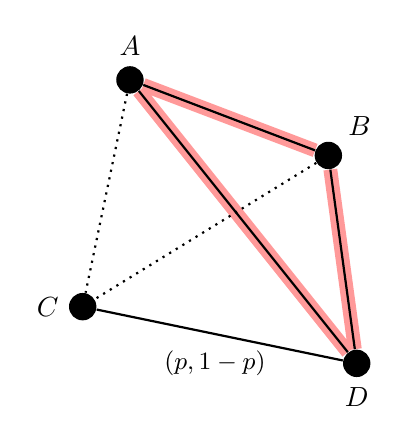
\begin{tikzpicture}[scale=1.2,v/.style={circle,fill=black,inner sep=3.5pt}]
\node[v,label=above:$A$] (A) at (0,2.4) {};
\node[v,label=above right:$B$] (B) at (2.1,1.6) {};
\node[v,label=left:$C$] (C) at (-0.5,0) {};
\node[v,label=below:$D$] (D) at (2.4,-0.6) {};
\draw[red!40,line width=5pt] (A)--(B)--(D)--(A);
\draw[thick] (A)--(B); \draw[thick] (A)--(D); \draw[thick] (C)--(D); \draw[thick] (B)--(D);
\draw[dotted,thick] (A)--(C); \draw[dotted,thick] (B)--(C);
\node[font=\small] at (0.9,-0.6) {$(p,1-p)$};
\end{tikzpicture}
\end{center}

\subsection*{حل}
\[
\Prob(\text{At least 1 }\Delta)=\Prob(ABC\cup ABD\cup ACD\cup BCD).
\]
\begin{itemize}
\item کلاً $\binom43=4$ مثلث می‌توانند رخ دهند: $ABC$، $ABD$، $ACD$ و $BCD$.
\item احتمال تشکیل هر یک از آن‌ها (به خاطر استقلال سه یال آن) برابر با $p\times p\times p=p^3$ است. یعنی داریم
\[\Prob(ABC)=\Prob(ABD)=\Prob(ACD)=\Prob(BCD)=p^3 .\]
\end{itemize}

\begin{question}[آیا می‌توان گفت $\Prob(\text{At least 1 }\Delta)=4p^3$ ؟]
\begin{answer}
\textbf{خیر، نمی‌توان گفت!} زیرا رخ دادن یک مثلث (مانند $ABC$) مانع رخ دادن یکی دیگر (مانند $BCD$) نمی‌شود. به عبارتی، این رخدادها ناسازگار (\lr{disjoint}) نیستند. پس احتمال اجتماع آنان برابر با جمعشان نیست. (البته طبق کران اجتماع، $4p^3$ یک \emph{کران بالا} است.)
\end{answer}
\end{question}

پس باید از \textbf{اصل شمول و عدم شمول} استفاده کنیم:
\begin{enumerate}
\item \textbf{اشتراک‌های دوتایی:} باید احتمالاتی مانند $\Prob(ABC\cap ABD)$ که دو بار شمرده شده‌اند کم شوند. تعداد این اشتراکات $\binom42=6$ است. از طرفی، هر دو مثلث متمایز در $K_4$ دقیقاً در یک یال مشترک‌اند (مثلاً $ABC$ و $ABD$ در یال $AB$)؛ پس هر اشتراک شامل رخ دادن دقیقاً ۵ یال مستقل است و احتمال هر یک برابر با $p^5$ است. تا بدین‌جا داریم: $4p^3-6p^5$.
\item \textbf{اشتراک‌های سه‌تایی:} سپس باید اشتراک‌های ۳تایی که زیادی کم شده‌اند، دوباره اضافه شوند. تعداد این اشتراکات $\binom43=4$ است، و در صورت بروز هر یک، تمام ۶ یال گراف می‌بایست رخ داده باشند (مثلاً $ABC$، $ABD$ و $ACD$ با هم همه ۶ یال را می‌پوشانند). پس احتمال هر یک $p^6$ است.
\item \textbf{اشتراک چهارتایی:} در نهایت، می‌بایست اشتراک ۴تایی (که یک حالت بیشتر ندارد) و دوباره مشتمل بر رخ دادن تمام یال‌های گراف است کم شود: $-p^6$.
\end{enumerate}
پس در نهایت خواهیم داشت:
\[
4p^3-6p^5+4p^6-p^6 ,
\]
یعنی
\[
\boxed{\ \Prob(\text{At least 1 }\Delta)=4p^3-6p^5+3p^6\ }
\]

\begin{note}
\notetitle \textbf{بررسی درستی:} به ازای $p=1$ گراف کامل است و جواب باید ۱ باشد: $4-6+3=1$ \checkmark. به ازای $p$های کوچک، جمله غالب $4p^3$ است؛ یعنی کران اجتماع در این حالت تقریب خوبی است (چون احتمال رخ دادن هم‌زمان دو مثلث، $O(p^5)$، بسیار کوچک‌تر است). این درستی را می‌توان با شمارش مستقیم همه $2^6=64$ حالت گراف نیز تأیید کرد.
\end{note}

\begin{center}
\begin{tikzpicture}
\begin{axis}[width=10cm,height=6cm,xlabel={$p$},ylabel={احتمال},xmin=0,xmax=1,ymin=0,ymax=1.2,legend pos=north west,legend style={font=\small},samples=100,domain=0:1]
\addplot[blue,very thick] {4*x^3-6*x^5+3*x^6};
\addlegendentry{\lr{exact: $4p^3-6p^5+3p^6$}}
\addplot[red,dashed,thick,domain=0:0.66] {4*x^3};
\addlegendentry{\lr{union bound: $4p^3$}}
\end{axis}
\end{tikzpicture}
\end{center}

\section{گراف‌های \lr{Erdős--Rényi} و مسئله تشکیل \lr{Clique}}

\begin{definition}[گراف تصادفی \lr{Erdős--Rényi}]
یک گراف تصادفی با $n$ رأس $V_1,\ldots,V_n$ در نظر بگیرید. هر یک از $\frac{n(n-1)}{2}$ یال بالقوه، مستقل از یکدیگر، با احتمال ثابت $p$ برقرار خواهند شد. به چنین گرافی، یک گراف تصادفی \lr{Erdős--Rényi} اطلاق می‌گردد و آن را با $G(n,p)$ نشان می‌دهیم.
\end{definition}

\begin{definition}[\lr{$r$-clique}]
به یک زیرگراف کامل (شامل تمام یال‌های دوبه‌دو) به سایز $r$ رأس (برای یک $2\le r\le n$)، یک \lr{$r$-clique} یا «خوشه $r$تایی» می‌گوییم. مثلث همان \lr{3-clique} است.
\end{definition}

\textbf{هدف:} یافتن کرانی برای احتمال تشکیل حداقل یک \lr{$r$-clique} در گراف، به ازای مقادیر ثابتی از $n,p,r$.

\subsection{کران بالا با کران اجتماع}
\begin{itemize}
\item احتمال تشکیل هر \lr{$r$-clique} مشخص (روی $r$ رأس معین) برابر است با
\[
\Prob(\text{one } r\text{-clique})=p^{\frac{r(r-1)}{2}},
\]
زیرا هر $r$ رأس، $\binom r2=\frac{r(r-1)}2$ یال دارند و همه باید (مستقلاً) برقرار باشند.
\item از طرفی، می‌دانیم که تعداد $\binom nr$ کلیک (مکان بالقوه) از سایز $r$ موجود هستند.
\item طبق کران اجتماع (\lr{Union Bound})، می‌توان یک کران بالا برای احتمال تشکیل حداقل یک \lr{$r$-clique} پیدا کرد:
\[
\boxed{\ \Prob(\text{At least one } r\text{-clique})\le\binom nr p^{\frac{r(r-1)}{2}}\ }
\]
\end{itemize}

\begin{note}
\notetitle محاسبه دقیق این احتمال با اصل شمول و عدم شمول (مانند حالت مثلث) بسیار پیچیده است، زیرا کلیک‌ها به شکل‌های مختلفی با هم هم‌پوشانی دارند. کران اجتماع با وجود سادگی، در بسیاری از کاربردها کافی است.
\end{note}

\subsection{ساده‌سازی کران}
\begin{theorem}[کران ضریب دوجمله‌ای]
برای $1\le r\le n$:
$\displaystyle\binom nr\le\Big(\frac{ne}{r}\Big)^r$.
\end{theorem}
\begin{proof}
$\binom nr=\frac{n(n-1)\cdots(n-r+1)}{r!}\le\frac{n^r}{r!}$. از طرفی از بسط تیلور $e^r=\sum_{k\ge0}\frac{r^k}{k!}\ge\frac{r^r}{r!}$، پس $r!\ge(r/e)^r$. با ترکیب این دو، $\binom nr\le n^r(e/r)^r$.
\end{proof}

برای ساده‌سازی بیشتر، با نوشتن $p=e^{-\log(1/p)}$ داریم:
\[
\Prob(\text{clique})\le\binom nr p^{\frac{r(r-1)}{2}}\le\Big(\frac{ne}{r}\Big)^r e^{-\frac{r(r-1)}{2}\log\left(\frac1p\right)}
=\exp\!\Big(r\Big[\log\frac{ne}{r}-\frac{r-1}{2}\log\frac1p\Big]\Big).
\]
با کمی عملیات جبری، می‌توان دید که در صورتی که داشته باشیم (فرمول ارائه‌شده در اسلاید)
\[
r\ \ge\ \frac{2\log(ne)}{\log(1/p)}+\frac{3}{\log(ne)},
\]
آنگاه احتمال تشکیل حداقل یک \lr{$r$-clique} (در رژیم معمول $n$ بزرگ) از مقدار $0.01$ کمتر است. نکته اصلی این است که \emph{بزرگ‌ترین کلیک یک گراف تصادفی، تنها از مرتبه $\frac{2\log n}{\log(1/p)}$ است.}

\begin{theorem}[یک شرط کافی دقیق]
اگر $r\ge4$ و $r\ge1+\dfrac{2\log(ne)}{\log(1/p)}$، آنگاه $\Prob(\text{At least one } r\text{-clique})\le r^{-r}\le\frac1{256}<0.01$.
\end{theorem}
\begin{proof}
از شرط دوم، $\frac{r-1}{2}\log\frac1p\ge\log(ne)$؛ پس عبارت داخل کروشه حداکثر $\log\frac{ne}{r}-\log(ne)=-\log r$ است و کران برابر $e^{-r\log r}=r^{-r}$ می‌شود. برای $r\ge4$ داریم $r^{-r}\le4^{-4}=\frac1{256}$.
\end{proof}

\begin{example}[مثال عددی]
برای $n=1000$ و $p=\frac12$، شرط بالا $r\ge1+\frac{2\log(1000e)}{\log2}\approx23.8$ می‌دهد. پس با احتمال بیش از ۹۹٪ هیچ کلیکی با ۲۴ رأس یا بیشتر در این گراف وجود ندارد؛ در حالی که گراف تقریباً $\frac12\binom{1000}{2}\approx250{,}000$ یال دارد! (محاسبه مستقیم کران $\binom{1000}{r}2^{-r(r-1)/2}$ نشان می‌دهد که حتی برای $r=20$ این احتمال کمتر از $10^{-15}$ است.)
\end{example}

\subsection{یک تخمین عددی ساده: شبکه‌های اجتماعی}
\begin{itemize}
\item در شبکه اجتماعی \lr{Facebook} یا \lr{Instagram} از قدر مرتبه $n=O(10^9)$ نفر عضو هستند.
\item تعداد متوسط «دوست»های هر عضو، از قدر مرتبه $np\approx O(10^3)$ است. (در گراف \lr{Erdős--Rényi} هر رأس به طور متوسط با $(n-1)p\approx np$ رأس دیگر همسایه است.) لذا داریم $p\approx O(10^{-6})$.
\item با جایگذاری در رابطه قبلی، می‌توان دید که در این صورت احتمال تشکیل کلیک‌هایی با $r\ge O(1)$ بسیار پایین است. به‌طور دقیق‌تر: $\frac{2\log(ne)}{\log(1/p)}\approx\frac{2\times21.7}{13.8}\approx3.1$؛ پس طبق قضیه بالا احتمال وجود حتی یک کلیک ۵تایی کمتر از $5^{-5}$ است. در واقع کران اجتماع برای $r=5$ مقدار $\binom{10^9}{5}10^{-60}\approx8\times10^{-18}$ را می‌دهد!
\end{itemize}

\begin{question}[آیا این عدد برای شما معقول است؟ به نظر شما ایراد کار از کجاست؟]
\begin{answer}
خیر، معقول نیست! در شبکه‌های اجتماعی واقعی، کلیک‌های بزرگ بسیار فراوان‌اند: اعضای یک خانواده، هم‌کلاسی‌ها، هم‌تیمی‌ها یا همکاران یک شرکت اغلب همگی با هم دوست‌اند و کلیک‌هایی با ده‌ها عضو می‌سازند.

ایراد در \textbf{مدل} است، نه در محاسبه. مدل \lr{Erdős--Rényi} دو فرض غیرواقعی دارد:
\begin{enumerate}
\item \textbf{استقلال یال‌ها:} در دنیای واقعی، اگر $X$ با $Y$ و $Y$ با $Z$ دوست باشد، احتمال دوستی $X$ و $Z$ بسیار بیشتر از حالت عادی است (پدیده «بستار سه‌گانه» یا \lr{triadic closure}). یعنی رخداد یال‌ها به شدت \emph{وابسته} است.
\item \textbf{همگنی:} احتمال $p$ برای همه جفت‌ها یکسان فرض شده، در حالی که افراد هم‌شهری، هم‌سن یا هم‌دانشگاهی با احتمال بسیار بیشتری دوست می‌شوند (ساختار اجتماعی یا \lr{community structure}).
\end{enumerate}
این مثال درس مهمی دارد: نتایج احتمالاتی فقط به اندازه فرض‌های مدل معتبرند. «فرض استقلال» یک فرض ساده‌کننده بسیار قوی است و باید با احتیاط به کار رود.
\end{answer}
\end{question}

\section{تمرین‌های تکمیلی}

\begin{exercise}
در مسئله دو سکه، $\Prob(C_2\given S_1)$ را برای $S_1=\mathtt{HHHHH}$ حساب کنید. سپس احتمال اینکه پرتاب بعدی شیر باشد (به شرط $S_1$) را بیابید.
\end{exercise}
\begin{solution}
درست‌نمایی‌ها: $\Prob(S_1\given C_1)=0.25^5\approx0.000977$ و $\Prob(S_1\given C_2)=0.8^5\approx0.32768$. با قانون بیز (پیشین‌های برابر):
\[
\Prob(C_2\given S_1)=\frac{0.32768}{0.32768+0.000977}\approx0.997 .
\]
با قانون احتمال کل شرطی و استقلال شرطی:
$\Prob(H\given S_1)=0.25\times0.003+0.8\times0.997\approx0.798$.
\end{solution}

\begin{exercise}
در گراف تصادفی با ۴ رأس، احتمال اینکه گراف \emph{هیچ} مثلثی نداشته باشد را برای $p=\frac12$ حساب کنید و با شمارش مستقیم تأیید کنید.
\end{exercise}
\begin{solution}
از فرمول: $1-(4p^3-6p^5+3p^6)$ و با $p=\frac12$: $4/8-6/32+3/64=\frac{32-12+3}{64}=\frac{23}{64}$؛ پس احتمال نبود مثلث $\frac{41}{64}$ است. شمارش مستقیم: با $p=\frac12$ همه $64$ گراف هم‌احتمال‌اند. گراف‌های دارای مثلث: با ۳ یال فقط ۴ گراف (خود مثلث‌ها)؛ با ۴ یال، هر مثلث به‌همراه یکی از ۳ یال دیگر: $4\times3=12$؛ با ۵ یال: هر ۶ گراف (حذف یک یال از $K_4$ فقط دو مثلث را خراب می‌کند)؛ با ۶ یال: ۱. جمع: $4+12+6+1=23$ \checkmark.
\end{solution}

\begin{exercise}
در گراف $G(n,p)$، با استفاده از کران اجتماع نشان دهید احتمال وجود دست‌کم یک رأس \emph{منزوی} (بدون هیچ یال) حداکثر $n(1-p)^{n-1}$ است. برای $n=100$ و $p=0.1$ این کران را حساب کنید.
\end{exercise}
\begin{solution}
رأس $i$ منزوی است اگر هیچ‌یک از $n-1$ یال آن برقرار نباشد؛ با استقلال احتمال آن $(1-p)^{n-1}$ است. با کران اجتماع روی $n$ رأس: $\Prob(\exists\text{ isolated})\le n(1-p)^{n-1}$. برای $n=100,p=0.1$: $100\times0.9^{99}\approx100\times2.95\times10^{-5}\approx0.003$.
\end{solution}
